\documentclass[final]{siamltex}

% for red MarginPars
\usepackage{color}

\usepackage{epsfig}
\usepackage{bm}

% total number of floats allowed on a page
\setcounter{totalnumber}{100}

% float page fractions
\renewcommand{\topfraction}{0.9}
\renewcommand{\bottomfraction}{0.9}
\renewcommand{\textfraction}{0.2}

% MarginPar
\setlength{\marginparwidth}{0.75in}
\newcommand{\MarginPar}[1]{\marginpar{\vskip-\baselineskip\raggedright\tiny\sffamily\hrule\smallskip{\color{red}#1}\par\smallskip\hrule}}

\def\eb  {{\bf e}}
\def\ib  {{\bf i}}
\def\nb  {{\bf n}}
\def\mRb {\bm{\mathcal{R}}}
\def\mZb {\bm{\mathcal{Z}}}

\def\half   {\frac{1}{2}}
\def\myhalf {\sfrac{1}{2}}

% for non-stacked fractions
\newcommand{\sfrac}[2]{\mathchoice
  {\kern0em\raise.5ex\hbox{\the\scriptfont0 #1}\kern-.15em/
   \kern-.15em\lower.25ex\hbox{\the\scriptfont0 #2}}
  {\kern0em\raise.5ex\hbox{\the\scriptfont0 #1}\kern-.15em/
   \kern-.15em\lower.25ex\hbox{\the\scriptfont0 #2}}
  {\kern0em\raise.5ex\hbox{\the\scriptscriptfont0 #1}\kern-.2em/
   \kern-.15em\lower.25ex\hbox{\the\scriptscriptfont0 #2}}
  {#1\!/#2}}

\begin{document}

%==========================================================================
% Title
%==========================================================================
\title{User's Guide to VARDEN}

\maketitle

\section{Introduction}
This is a working design document for the VARDEN code.  VARDEN
solves the variable-density incompressible Navier-Stokes equations using
a finite volume, AMR framework.  See \cite{Almgren:1998}
for a description of the algorithm.
Note that VARDEN does not subcycle in time, i.e., all the levels are integrated
in time with the same time step.

\section{Source Code}
There are two git repositories required to build/run the code.  amrex is available on
github but is not public yet (contact Andy Nonaka {\tt ajnonaka@lbl.gov}
to obtain access).\\ \\
VARDEN is available on github and can be obtained using the command:\\ \\
{\tt git clone https://github.com/BoxLib-Codes/VARDEN.git}\\ \\
You will now have the following directory structures (you will actually have
more subdirectories, but below are the only directories that matter for this code):\\
%%%%%%%%%%%%%%%%%%%%%%%%%%%%%%%%%%%%%
\begin{figure}[tb]
\centering
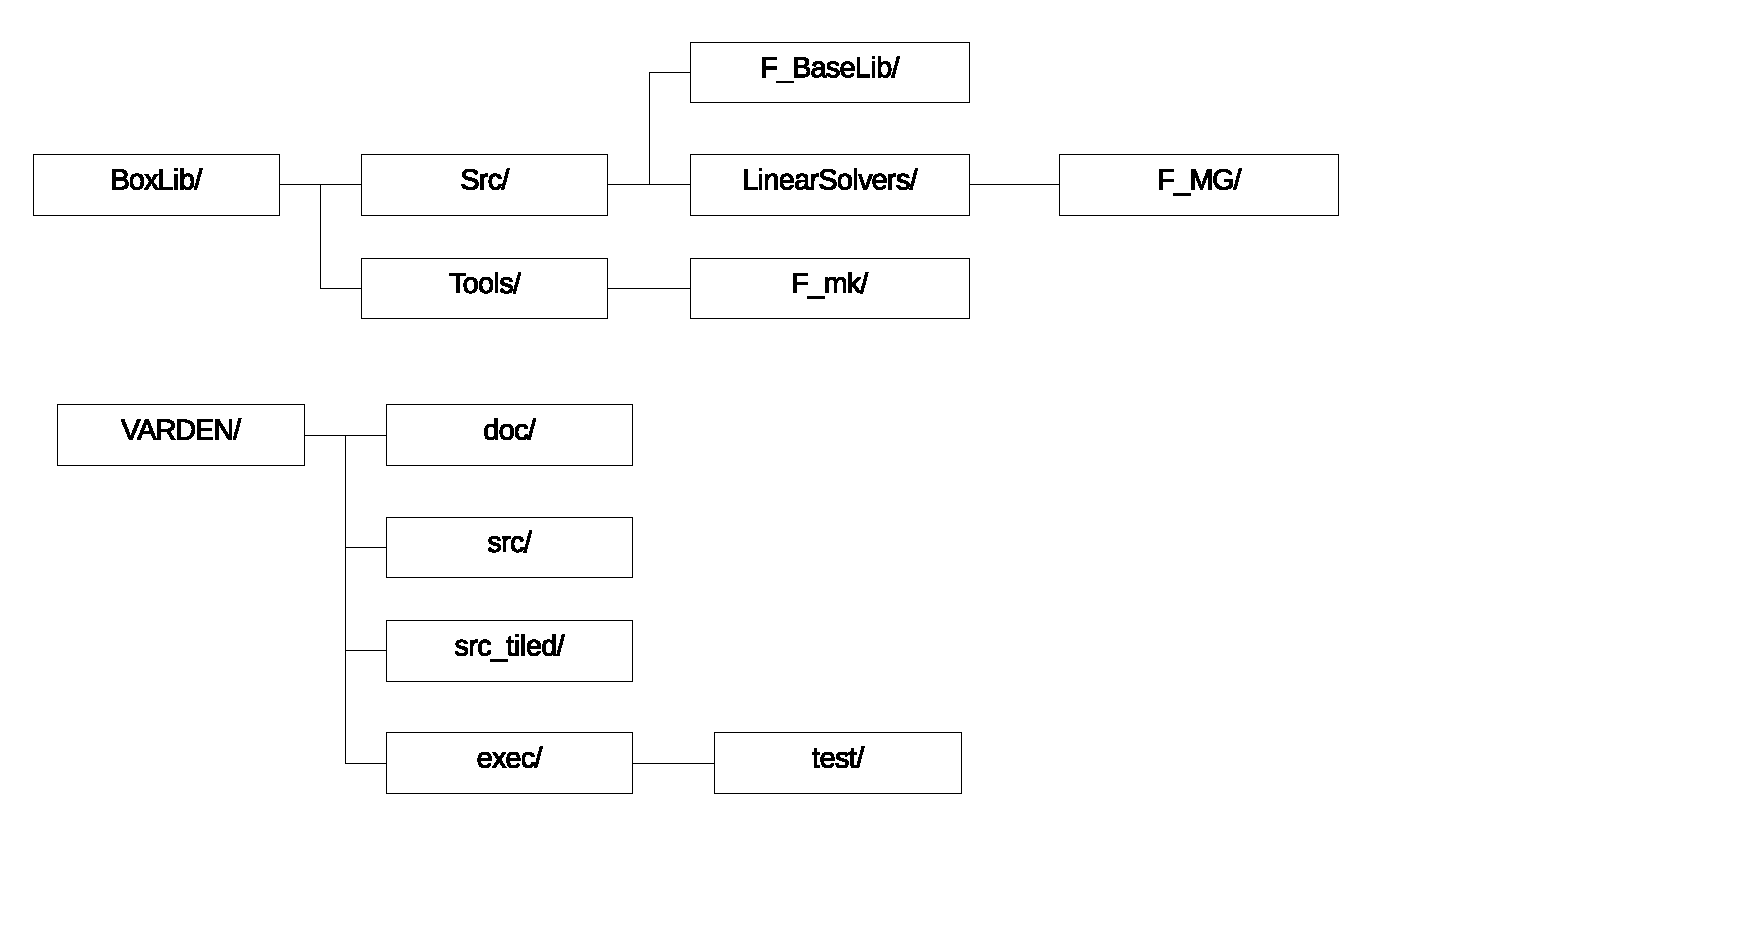
\includegraphics[width=6in]{./directory}
\caption{\label{fig:directory}Directory structure.}
\end{figure}
%%%%%%%%%%%%%%%%%%%%%%%%%%%%%%%%%%%%%
\begin{itemize}

\item {\tt amrex/}

\begin{itemize}

\item {\tt Src/}

\begin{itemize}

\item {\tt F\_BaseLib/}

Core libraries for parallelization of structured grid data.

\item {\tt LinearSolvers/F\_MG/}

Core libraries for linear solvers (for implicit diffusion) and diffusion stencils.

\end{itemize}
\end{itemize}

\begin{itemize}

\item {\tt Tools/F\_mk/}

Make system variables and flags.

\end{itemize}
\end{itemize}

\begin{itemize}

\item {\tt VARDEN/}

\begin{itemize}

\item {\tt doc/}

Documentation.  Contains this User's Guide.

\item {\tt src/}

VARDEN source code

\item {\tt src\_tiled/}

A tiled version of the source code (a more efficient OpenMP implementation for
manycore architectures).  More info on this soon.

\item {\tt exec/test/}

The build directory.

\end{itemize}
\end{itemize}

\subsection{Compiling and Running}
Go to {\tt VARDEN/exec/test/} and edit the 
{\tt GNUmakefile} settings to your liking (below) and simply type {\tt `make'}.\\
\begin{verbatim}
NDEBUG    :=           # 'not debug'.  use 't' for an optimized build
MPI       := t         # use 't' to build an mpi executable
OMP       :=           # use 't' to build an OpenMP threadded executable
PROF      :=           # use 't' to turn on code profiling
COMP      := gfortran  # fortran compiler
CCOMP     := gcc       # c compiler
TILING    :=           # enable tiled OpenMP version of the code

\end{verbatim}
This will generate an executable whose name provides information about the build settings,
i.e., what compiler was used, whether MPI and/or OpenMP were enabled, etc.
To run the code, simply type the executable name, followed by an inputs file.

\subsection{Input Parameters}
Refer to {\tt src/probin.f90} for namelist parameters used in the
simulation and an explanation of what the parameters do.

\bibliographystyle{plain}
\bibliography{DesignDocument}

\end{document}
